\documentclass{beamer}
\usepackage{listings}
\usepackage{verbatim}
\usepackage{minted}
\usepackage{svg}
\usepackage[space]{grffile}


\usepackage{pgfpages}
%\setbeameroption{show notes}
%\setbeameroption{show notes on second screen=right}

\definecolor{codegreen}{rgb}{0,0.6,0}
\definecolor{codegray}{rgb}{0.5,0.5,0.5}
\definecolor{codepurple}{rgb}{0.58,0,0.82}
\definecolor{backcolour}{rgb}{0.95,0.95,0.92}
\lstdefinestyle{mystyle}{
    backgroundcolor=\color{backcolour},
    keywordstyle=\color{magenta},
    stringstyle=\color{codepurple},
    basicstyle=\ttfamily\footnotesize,
    breakatwhitespace=false,
    breaklines=true,                 
    captionpos=b,                    
    keepspaces=true,                  
    numbersep=1pt,                  
    showspaces=false,                
    showstringspaces=false,
    showtabs=false,                  
    tabsize=2,
    language=bash,
    numbers=left,
    stepnumber=1,    
  firstnumber=1,
  numberfirstline=true
}
\lstset{style=mystyle}


%\setminted{fontsize=\footnotesize}
%\lstset{basicstyle=\ttfamily,breaklines=true}


\usetheme{Boadilla}

\title{Git Tutorial}
\subtitle{How to git for fun \& profit }
\author{Thomas Dost}
\date{\today}



\beamertemplatenavigationsymbolsempty

\titlegraphic{
\includegraphics[width=.3\textwidth,height=.3\textheight]{memes/understand_git.jpg}}


\begin{document}

\begin{frame}
\titlepage
\end{frame}

\begin{frame}[fragile,t]{What is git}
  \begin{columns}
    \begin{column}{0.5\textwidth}
      \begin{enumerate}
        \item version control system
        \item a version control sytem is a system that records changes to a set of files over time so that you can recall specific versions later
      \end{enumerate}
    \end{column}

    \begin{column}{0.5\textwidth}
      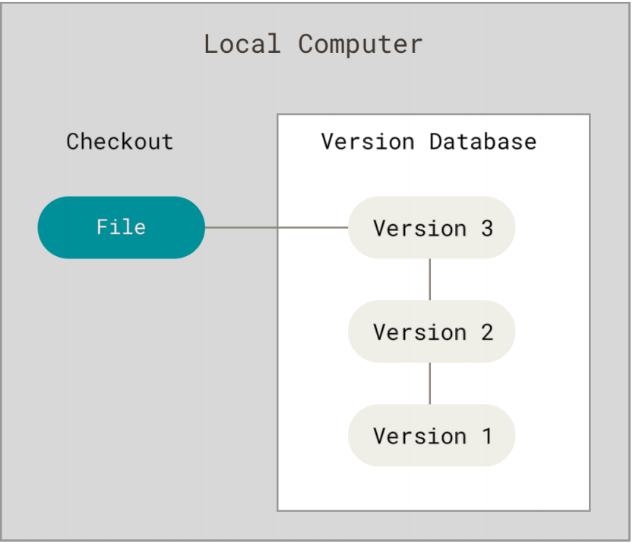
\includegraphics[width=0.9\textwidth,height=0.6\textheight]{screenshots/2022-03-27-110459_634x543_scrot.png}
    \end{column}
  \end{columns}
\end{frame}


\begin{frame}[fragile,t]{Centralized version control vs distributed version control}
  \begin{columns}
    \begin{column}{0.5\textwidth}
      \begin{enumerate}
        \item all files are stored on a central server
        \item each developer can checkout a specific file, which makes other developers unable to edit it as well
      \end{enumerate}\vspace{10pt}

      \begin{enumerate}
        \item each developer has local copy of all the files
        \item most operations are local, i.e. each developer can work idependently of the the others
        \item everything you do in git is checksumed, that means its impossible to change anything without Git knowing about it
      \end{enumerate}

    \end{column}
    \begin{column}{0.5\textwidth}
      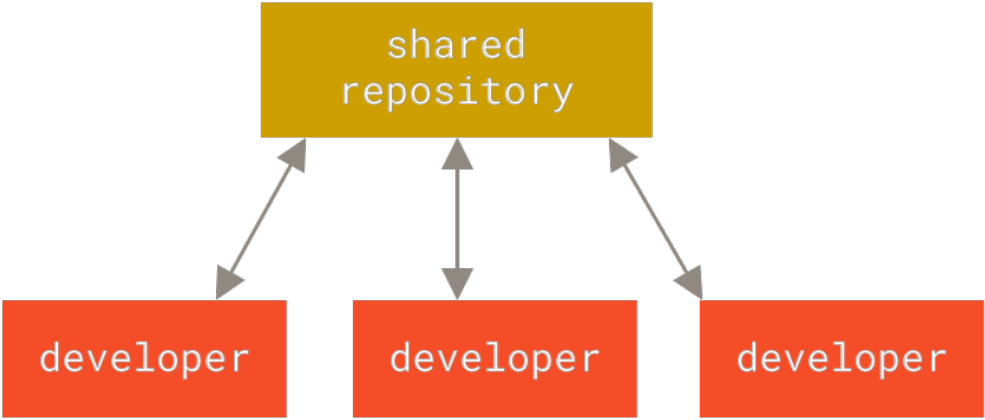
\includegraphics[width=0.9\textwidth,height=0.3\textheight]{screenshots/2022-03-27-110945_985x420_scrot.png}
      \centering
      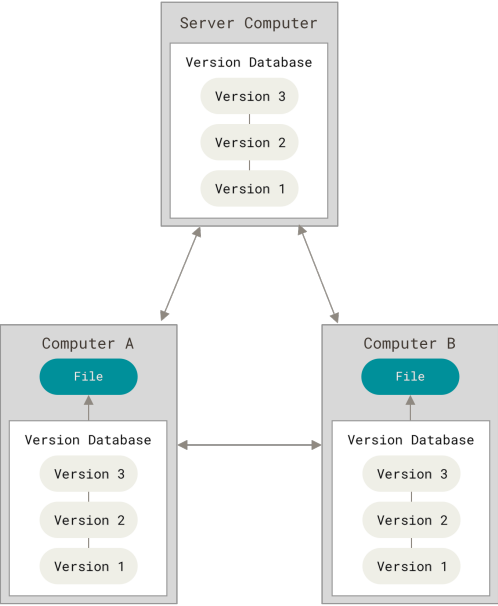
\includegraphics[width=0.6\textwidth,height=0.6\textheight]{screenshots/2022-03-27-111452_498x606_scrot.png}
    \end{column}
  \end{columns}
\end{frame}



\begin{frame}[fragile,t]{Three stages of git }
  \begin{center}
    \centering
  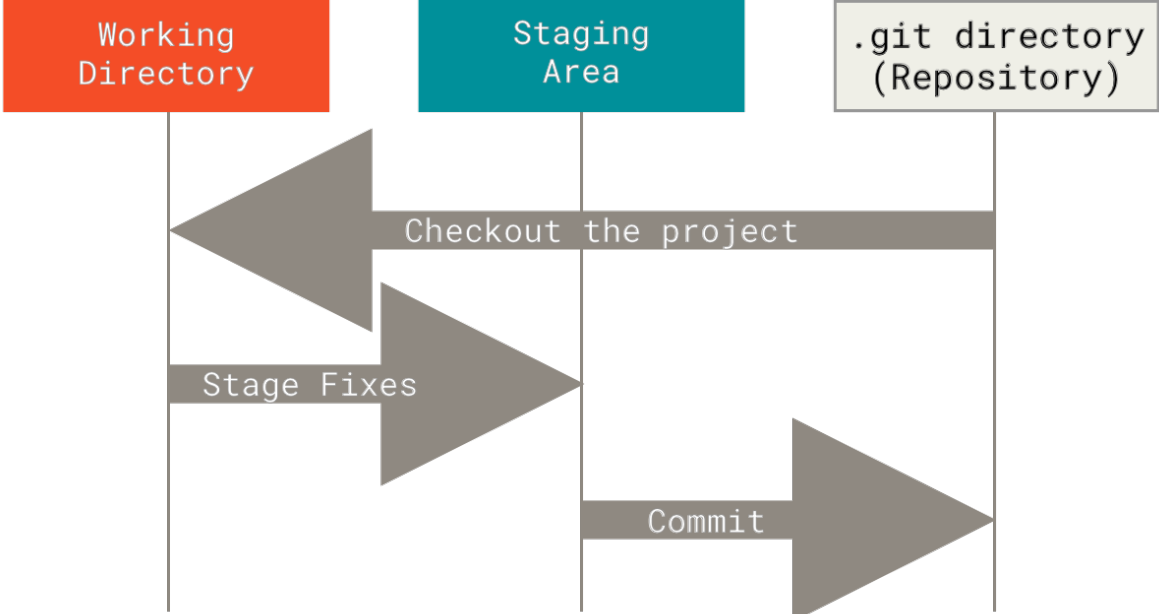
\includegraphics[width=0.8\textwidth,height=0.7\textheight]{screenshots/2022-03-27-113647_1159x614_scrot.png}
  \end{center}
\end{frame}

\begin{frame}[fragile,t]{Setting up git}
  \textbf{Prerequisite:} Some version of git should be installed(in my case it's 2.30.2)\vspace{10pt}
  
  
  \textbf{Git config paths}
  \note{Possible paths to put git config files}
  \begin{itemize}
    \item \textcolor{magenta}{~/.gitconfig} 
    \item \textcolor{magenta}{~/.config/git/config}
    \item \textcolor{magenta}{.git/config}
  \end{itemize} 
  \vspace{10pt}
  \textbf{Show current config}
  \begin{lstlisting}
  git config --list --show-origin
  git config  user.name "Thomas Dost"
  git config  user.email ThomasDost@example.com
  git config  core.editor vim\end{lstlisting}
  \note{use those commands to set your stuff, note that the your can use the the local config overwrites the global one}
  \note{the last command changes the default editor git \textcolor{red}{do example}}
  \vspace{10pt}
  \textbf{Getting help}
  \begin{lstlisting}
  git help <command>\end{lstlisting}
  \note{e.g commit or config}
\end{frame}




\begin{frame}[fragile,t]{Making a new repository}
  \textbf{New repository}
  \begin{lstlisting}
  git init
  git init <name>\end{lstlisting}

  \textbf{Cloning an existing repository}
  \begin{lstlisting}
  git clone <url>\end{lstlisting}\pause

  \note{make new file main.py| touch main.py}
  \note{main.1.py}
  \note{chmod +x main.py}
  \textbf{Adding files to the staging area}
  \begin{lstlisting}
  git add main.py \end{lstlisting}\pause
  \note{to repostiry| git add main.py}
  \note{show status | git status}
  \note{only in staging area, not commited}
  \textbf{Committing changes}
  \begin{lstlisting}
  git commit main.py \end{lstlisting}\pause
  \note{Opens editor to write commit message}

  \note{\textcolor{red}{ADD FEATURE TO PYTHON PROGRAM}}

  \textbf{Amending/Verbose}
  \begin{lstlisting}
  git commit -a main.py #amend a commit
  git commit -v main.py #show difference\end{lstlisting}
  \note{enables you edit last commit message}
  \note{shows diff}
\end{frame}



\begin{frame}[fragile,t]{Interactive adding}\vspace{10pt}
  \begin{lstlisting}
  git add -p \end{lstlisting}
  \begin{itemize}
    \item \textcolor{magenta}{-y} stage the chunk
    \item \textcolor{magenta}{-n} ignore the chunk
    \item \textcolor{magenta}{-s} split into smaller chunks
    \item \textcolor{magenta}{-e} edit the chunk
    \item \textcolor{magenta}{-q} exit
  \end{itemize}

  \note{later make this easier}
\end{frame}

\begin{frame}[fragile,t]{Look back in time(git log)}\vspace{10pt}
  \begin{lstlisting}
  git log \end{lstlisting}
  \begin{itemize}
    \item \textcolor{magenta}{--graph } 
    \item \textcolor{magenta}{--oneline} 
    \item \textcolor{magenta}{--decorate} 
  \end{itemize}
\end{frame}


\begin{frame}[fragile,t]{Look back in time(git log)}\vspace{10pt}
  \begin{lstlisting}
  git diff\end{lstlisting}
  \note{does not show diffs of already staged aka. commited files}
  \begin{itemize}
    \item \textcolor{magenta}{--staged} also diff files which are already staged
  \end{itemize}
  \note{show how to compare diff of two commits}
  \begin{lstlisting}
  git difftool\end{lstlisting}
\end{frame}


\begin{frame}[fragile,t]{Checking out older commits}\vspace{10pt}
  \begin{columns}
    \begin{column}{0.5\textwidth}
      \begin{lstlisting}
  git checkout <commit-id>\end{lstlisting} 

      \end{column}
    \begin{column}{0.5\textwidth}
      
\includegraphics[width=1\textwidth,height=0.5\textheight]{memes/detached_head.jpg}
    \end{column}
  \end{columns}
  \note{detached head -> later} 
  \note{how we can use this to find bugs}
  \note{compares the already commited stages with the specified commit}
\end{frame}

%TODO Look at this again
\begin{frame}[fragile,t]{Reverting changes/Cleaning up}\vspace{10pt}
  revert unstaged changes
  \begin{lstlisting}
  git restore <file>\end{lstlisting}\vspace{10pt}

  reset all staged changes
  \begin{lstlisting}
  git reset HEAD \end{lstlisting}\vspace{10pt}
  
  revert last commit
  \begin{lstlisting}
  git revert HEAD\end{lstlisting}\vspace{10pt}
  
  Remove directories
  \begin{lstlisting}
  git rm\end{lstlisting}\vspace{10pt}
  
  Remove all files not under gits control
  \begin{lstlisting}
  git clean\end{lstlisting}\vspace{10pt}
\end{frame}

\begin{frame}[fragile,t]{git revert}\vspace{10pt}
  reverts and already committed change by inverting it and appending a new comit
  \begin{lstlisting}
  git revert <commit-hash>\end{lstlisting}\vspace{10pt}
  \begin{itemize}
    \item \textcolor{magenta}{-n}, does not create a new commit, instead stages the changes
  \end{itemize} 
\end{frame}


\begin{frame}[fragile,t]{git reset}\vspace{10pt}
  Three primary modes of invocation, which correspond to gits internal management stages. Mostly used to remove files from the staging area
  \begin{itemize}
    \item \textcolor{magenta}{--soft}: the commit tree(HEAD)
    \item \textcolor{magenta}{--mixed}: the staging index
    \item \textcolor{magenta}{--hard}: the working directory
  \end{itemize} 

  \begin{lstlisting}
  git reset # remove all files from staging area
  git reset <file> # removes <file> from statging area
  git reset --hard  \end{lstlisting}\vspace{10pt}
  \textcolor{red}{ --hard undoes all uncommited changes}

\end{frame}

\begin{frame}[fragile,t]{git revert vs. git reset}\vspace{10pt}
  \note{It's important to understand that git revert undoes a single commit—it does not "revert" back to the previous state of a project by removing all subsequent commits. In Git, this is actually called a reset, not a revert.}
  \begin{columns}
    \begin{column}{0.5\textwidth} 
      \textbf{reverting} does not change the history i.e. its safe.\vspace{10pt}\\
      \textbf{git revert} is able to target arbitrary commits in the history, while reset only works backwards from the current commit
    \end{column}
    \begin{column}{0.5\textwidth} 
      \centering
      \includesvg[width=0.9\textwidth,height=0.9\textheight]{screenshots/reset}
    \end{column}

  \end{columns}
\end{frame}

\begin{frame}[fragile,t]{Branching 1}\vspace{10pt}
  \note{ets say you want to implement a new feature which will take a while and might leave your program in an "unusable" state, but you still want to be able to run the current version of your program. There ofc is a feature for that called branching}
  \begin{columns}
    \begin{column}{0.5\textwidth} \includegraphics[width=0.9\textwidth,height=0.6\textheight]{"screenshots/Pasted image 20220326155633"} \end{column}

    \begin{column}{0.5\textwidth}
      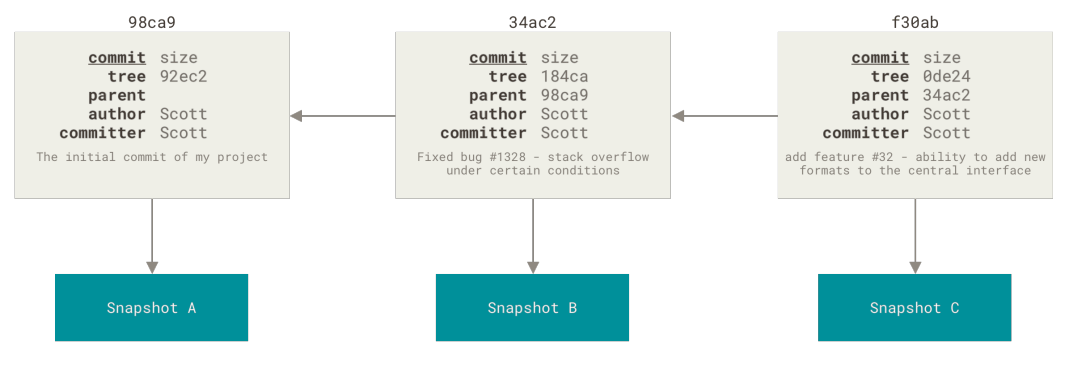
\includegraphics[width=\textwidth,height=0.3\textheight]{screenshots/2022-03-27-100919_1069x370_scrot.png}
    \end{column}
  \end{columns}

\end{frame}


\begin{frame}[fragile,t]{Creating a branch}\vspace{10pt}
  \begin{columns}
    \begin{column}{0.5\textwidth}
      \begin{lstlisting}[basicstyle=\ttfamily\tiny]
  git branch <branch-name> # create branch\end{lstlisting}\vspace{30pt}


      \begin{lstlisting}[basicstyle=\ttfamily\tiny]
  git checkout <branch-name> #switch to branch
  git checkout -b <branch-name> #create and switch \end{lstlisting}\vspace{10pt}
    \end{column}

    \begin{column}{0.5\textwidth}
      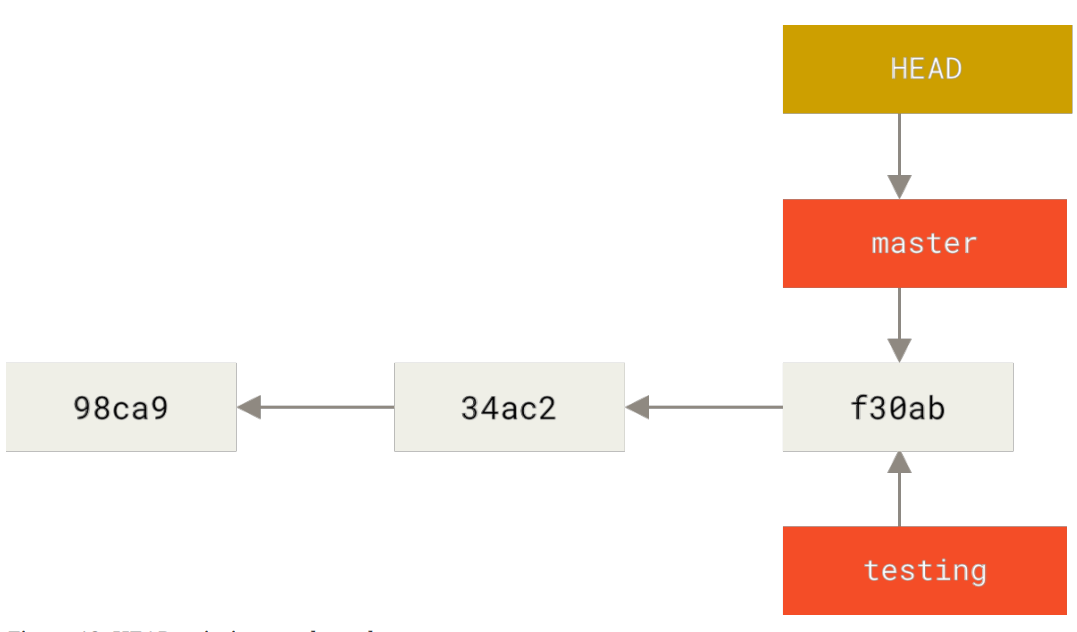
\includegraphics[width=\textwidth,height=0.3\textheight]{screenshots/2022-03-27-102830_1077x632_scrot.png}\vspace{20pt}
      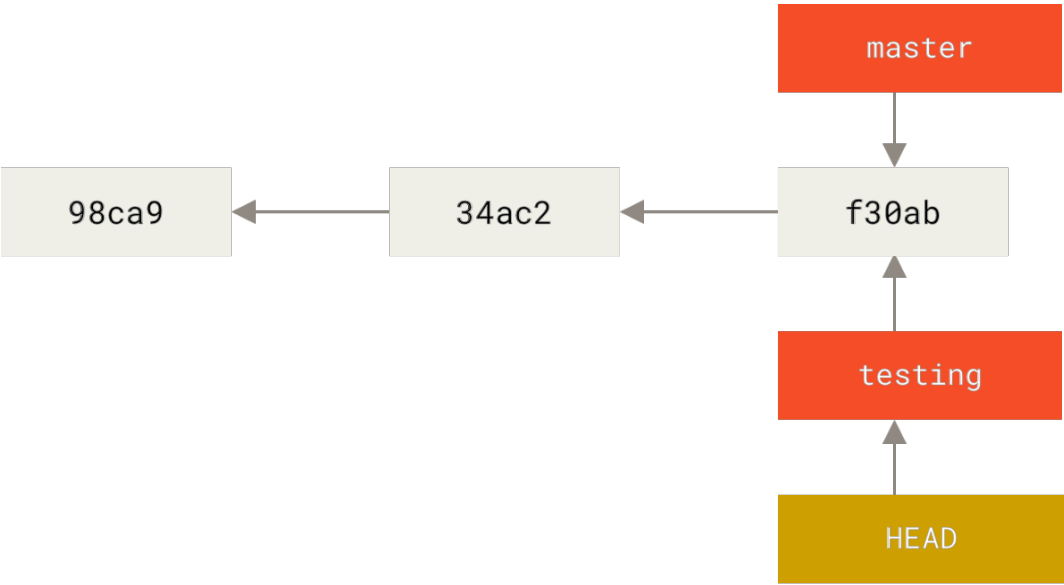
\includegraphics[width=\textwidth,height=0.3\textheight]{screenshots/2022-03-27-103033_1064x585_scrot.png}
    \end{column}
    \note{ branch in Git is simply a lightweight movable pointer to one of these commits. The default branch name in Git is master. As you start making commits, you’re given a master branch that points to the last commit you made. Every time you commit, the master branch pointer moves forward automatically How does Git know what branch you’re currently on? It keeps a special pointer called HEAD. Note that this is a lot different than the concept of HEAD in other VCSs you may be used to, such as Subversion or CVS.}
  \end{columns}

  \note{git checkout -b feature/user}
  \note{example main.3.py }
  \note{git log --all --graph}

\end{frame}

\begin{frame}[fragile,t]{Merging}\vspace{10pt}
  \note{checkout main again and show that there are now changes}
  \note{git checkout main}
  \note{git merge feature/user}
  %TODO
  \begin{lstlisting}[basicstyle=\ttfamily\tiny]
  git checkout main
  git merge <other-branch> # merges the other branch onto main
  git branch -d feature/user # safe delete\end{lstlisting}\vspace{10pt}

  \begin{columns}
    \begin{column}{0.5\textwidth}
      \begin{figure}
        \centering
        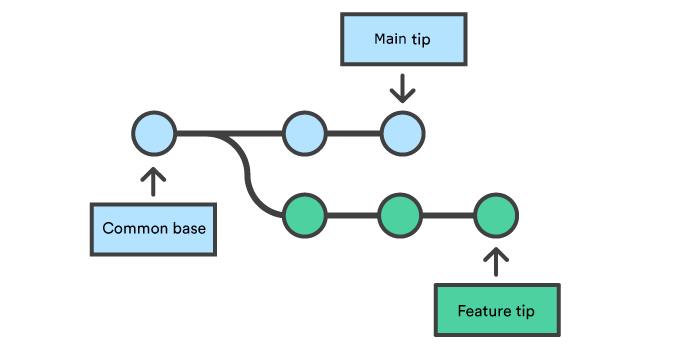
\includegraphics[scale=0.2]{screenshots/merge.png}
        \caption{Before a merge}
      \end{figure}
    \end{column}

    \begin{column}{0.5\textwidth}
      \begin{figure}
        \vspace{-15pt}
        \centering
        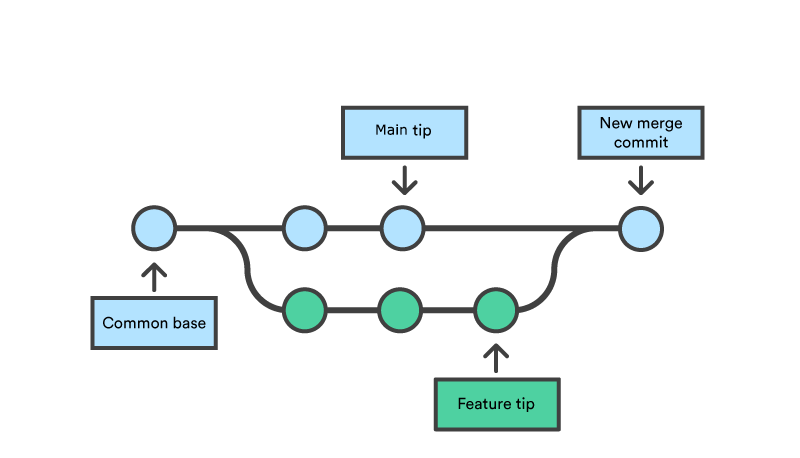
\includegraphics[scale=0.2]{screenshots/merge2.png}
        \caption{After a merge}
      \end{figure}
    \end{column}
  \end{columns}
  \note{does not work if there still are uncommited changes}
\end{frame}

\begin{frame}[fragile,t]{Collaboration}\vspace{10pt}
  We now know how to 
  \begin{enumerate}
    \item execute basic git commands
    \item work with branches
  \end{enumerate}\vspace{10pt}
  But everything we did was local, so how do we work online or with other people via git?

  \begin{lstlisting}[basicstyle=\ttfamily\tiny]
  git push # upload local changes
  git pull # download changes and merge into branches\end{lstlisting}\vspace{10pt}

  \note{Those are the basics of working locally. But you are probably asking yourself: Whats up with GitLab and GitHub and how can I backup my files, because atm all of our files are still only stored on our local computer i.e. if the drive fails all of our data is gone. So lets talk about GitLab}
  \note{open git hub}
  \note{push changes}
\end{frame}


\begin{frame}[fragile,t]{Merge conflicts}\vspace{10pt}
  What happens when we make conflicting changes?


\end{frame}

\begin{frame}[fragile,t]{.gitignore}\vspace{10pt}
  Used to specify specific files, file endings which git should ignore, also possible to ignore whole folders
  \note{make a few files with a specific endings}
  \note{make a directory, with files which should get igored}
\end{frame}

\begin{frame}[fragile,t]{git tag}\vspace{10pt}
  \begin{lstlisting}
  git tag # list all tags
  git tag -a <tag-name> -m "<message>" # annotaged tag
  git tag <tag-name> # lightweight tag

  git tag <tag-name> <commit-id> # add tag to earlier commit
  git push --tags # by defaults tags are not pushed
  git tag -d <name> # delete tag
  git checkout <tag-name> #go to specific commit by tag name\end{lstlisting}
  \note{git checkout -b <branch-name> <tag-name>}
\end{frame}

\begin{frame}[fragile,t]{Stashing}\vspace{10pt}
  What happens when you in the middle of changing sth., and for example, a colleague wants you to look at the stuff he just did.
  \begin{lstlisting}
  git stash #
  git stash pop\end{lstlisting}
\end{frame}


\begin{frame}[fragile,t]{Git \& RStudio}\vspace{10pt}
\end{frame}

\begin{frame}[fragile,t]{Versioning}\vspace{10pt}
  no standard way of when/what to commit
  commit \textcolor{magenta}{semantically} similiar units\vspace{10pt}

  \textbf{SemVer}
  \textbf{Prerequisite}: A version number in the form of MAJOR.MINIOR.PATCH
  Change 
  \begin{enumerate}
      \item MAJOR version when you make incompatible API changes
      \item MINOR version when you add functionality in a backwards compatible manner
      \item PATCH version when you make backwards compatible bug fixes
  \end{enumerate}\vspace{10pt}
  All of those, of course, warrant a commit but are not really applicable outside of software engineering

  There is a another workflow based on rebase, which enables you to basically just commit everything%TODO Is this true
\end{frame}

\begin{frame}[fragile,t]{git rebase}\vspace{10pt}
  Combines older/multiple commits into one base commit.\vspace{10pt}\\
  Alleviates the issue of what/when to commit\vspace{10pt}\\
  Do \textcolor{red}{NOT} use in public repositories/already published changes. There are workflows to mitigate this risk

  \begin{lstlisting}
  git rebase -i\end{lstlisting}

\end{frame}

\begin{frame}[fragile,t]{git difftools}\vspace{10pt}
\end{frame}

\begin{frame}[fragile,t]{Tools}\vspace{10pt}
  \begin{enumerate}
    \item GitKraken(Partially free)
      \item GitHub Desktop(free)
    \item Magit{Emacs}(free)
    \item SourceTree(free)
  \end{enumerate}
\end{frame}


\begin{frame}[fragile,t]{Things not covered}\vspace{10pt}
  \begin{enumerate}
    \item git lfs: git large file storage
    \item git merge in-depth: understanding what merge does exactly is pretty usefull when working with it
    \item git rebase: "alternative" to merge, allows a linear commit history %https://www.youtube.com/watch?v=f1wnYdLEpgI&ab_channel=TheModernCoder
    \item git rebase: Changing history %https://www.youtube.com/watch?v=9y9IRBKDU4I&ab_channel=raywenderlich.com
    \item git rebase vs merge: rebase allows a cleaner history
    \item git workflows: automatic running of tests and deployment i.e. publishing to pip or stuff like that
    \item forking: how copy other open source project and contribute to them -> leads to pull requests
    \item git blame: who/what was modified on a specific file
  \end{enumerate}
\end{frame}

\begin{frame}[fragile,t]{Things not covered}\vspace{10pt}
  \begin{enumerate}
      \setcounter{enumi}{8}
    \item git hooks: run user scripts at specific git events(server/client side)
    \item git cherrypick
    \item git submodules: incorporate external code https://www.atlassian.com/git/tutorials/git-submodule
    \item git subtrees: alternative to git submodules
    \item git reflog: Allows you to visit commits, which are not referenced by any brach anymore, for example after a squash
    \item git bisect:  "automatic" bug finding, requires tests
    \item git alias: Make "shortcuts" for git commands
  \end{enumerate}
\end{frame}


\begin{frame}[fragile,t]{Warning}\vspace{10pt}
  A lot of the commands which change the history have to be used with caution if you work on a public repo. with other developers, please read up/think about what happens when your change local history referenced by other developers and try to push those changes, but that is out of the scope for this presentation.
  \begin{figure}
      \centering
      
\includegraphics[width=0.5\textwidth,height=0.5\textheight]{memes/with-great-power.jpg}

  \end{figure}
\end{frame}

\begin{frame}[fragile,t]{References}\vspace{10pt}
  \begin{enumerate}
    \item https://git-scm.com/site(All material under MIT)
    \item ProGit(All material under CreativeCommons CC-BY-NC-SA)
    \item Atlassian tutorials(Just stolen :'), no license given)
    \item https://semver.org/lang/en/
  \end{enumerate}
\end{frame}

\begin{frame}{Questions?}
  \centering
      
\includegraphics[width=0.7\textwidth,height=0.7\textheight]{memes/git_awesome.jpg}
\end{frame}
\end{document}



  %j\begin{block}
    %dwdwd
  %\end{block}
